%! alt Two equal circles with centres A and B, each passing through the other's centre, meet at E. C is the second point where line AB meets the circle centred at A, and P lies on arc CE away from B. Triangle ABE is equilateral with a 60 degree angle at E, triangle AEP is isosceles with AE = AP and apex angle theta at A, and segment EP is highlighted.
%! after_paragraph 2
%! scale 1
% The shared preamble of every Cevian figure. pipeline/figures turns these colours into theme-aware paint,
% and refuses any other colour, so draw only with them:
%   figink (lines and labels), figaux (construction lines), figaccent (the object the argument turns on),
%   figtint and figaccenttint (light fills).
\documentclass[border=1.5pt]{standalone}
\usepackage{tkz-euclide}
\definecolor{figink}{RGB}{0,0,0}
\definecolor{figaux}{RGB}{85,85,85}
\definecolor{figaccent}{RGB}{192,57,43}
\definecolor{figtint}{RGB}{221,221,221}
\definecolor{figaccenttint}{RGB}{245,213,208}
% tkz-euclide's defaults draw circles, compasses and marks in 50% grey and fill points with a tint.
\makeatletter
\def\tkz@otherlinecolor{figink}
\def\tkz@euc@circlecolor{figink}
\def\tkz@euc@compasscolor{figink}
\def\tkz@euc@mkcolor{figink}
\def\tkz@mk@fill{figink}
\def\tkz@euc@pointfillcolor{figink}
\makeatother
\tkzSetUpLine[color=figink,line width=.7pt]
\tkzSetUpArc[color=figink,line width=.7pt]
\tkzSetUpCompass[color=figink,line width=.5pt]
\tkzSetUpPoint[color=figink,fill=figink,size=3.1pt]
\tikzset{
  every picture/.style={line cap=round,line join=round,color=figink},
  circle style/.append style={color=figink,line width=.7pt},
  aux/.style={color=figaux,line width=.45pt,dash pattern=on 2.6pt off 2pt},
  key/.style={color=figaccent,line width=1pt},
  mk/.style={color=figink,line width=.5pt},
  lbl/.style={color=figink,inner sep=2.2pt},
  len/.style={color=figink,inner sep=1.5pt,font=\small},
}

\begin{document}
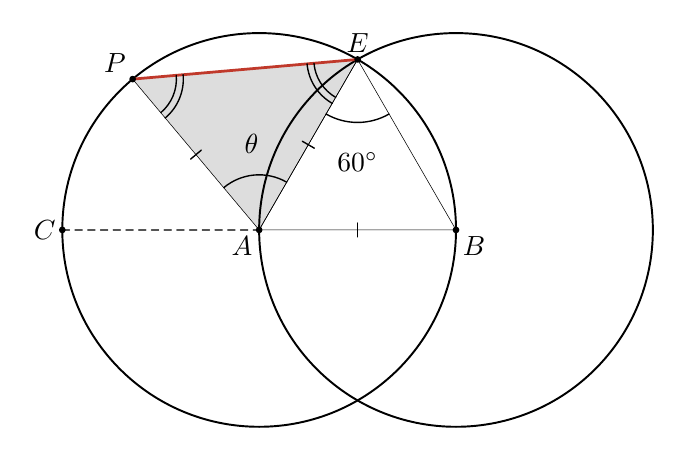
\begin{tikzpicture}
%! let R = 5/2
\tkzDefPoint(0.0,0.0){A} %! A = (0, 0)
\tkzDefPoint(2.5000000,0.0){B} %! B = polar(A, R, 0)
\tkzDefPoint(-2.5000000,0.000000000000000000000000000000000000000000000000010837084){C} %! C = polar(A, R, 180)
\tkzDefPoint(1.2500000,2.1650635){E} %! E = polar(A, R, 60)
\tkzDefPoint(-1.6069690,1.9151111){P} %! P = polar(A, R, 130)
%! fact on_circle(B, A, R)
%! fact on_circle(A, B, R)
%! fact on_circle(E, A, R)
%! fact on_circle(E, B, R)
%! fact on_circle(C, A, R)
%! fact on_circle(P, A, R)
%! fact on_segment(A, B, C)
%! fact equal(dist(A, E), dist(A, P))
%! fact angle(B, E, A) == 60
%! fact angle(E, A, C) == 120
%! example angle(E, A, P) <= 120
%! example angle(B, E, P) >= 90
\tkzFillPolygon[color=figtint](A,E,P)
\tkzDrawCircle(A,B)
\tkzDrawCircle(B,A)
\tkzDrawSegment[aux](C,A)
\tkzDrawPolygon(A,B,E)
\tkzDrawPolygon(A,E,P)
\tkzDrawSegment[key](E,P)
\tkzMarkSegments[mark=|,size=2.5pt,mk](A,B A,E A,P)
\tkzMarkAngle[size=.8,arc=l,mark=none,mk](A,E,B)
\tkzMarkAngle[size=.6,arc=ll,mark=none,mk](P,E,A)
\tkzMarkAngle[size=.6,arc=ll,mark=none,mk](A,P,E)
\tkzMarkAngle[size=.7,arc=l,mark=none,mk](E,A,P)
\tkzDrawPoints(A,B,C,E,P)
\tkzLabelPoint[below left,lbl](A){$A$}
\tkzLabelPoint[below right,lbl](B){$B$}
\tkzLabelPoint[left,lbl](C){$C$}
\tkzLabelPoint[above,lbl](E){$E$}
\tkzLabelPoint[above left,lbl](P){$P$}
\tkzLabelAngle[pos=1.3](A,E,B){$60^\circ$}
\tkzLabelAngle[pos=1.1](E,A,P){$\theta$}
\end{tikzpicture}
\end{document}
